% Figure 1: CHE System Architecture
% Standalone TikZ figure for Paper 3
\documentclass[tikz,border=5pt]{standalone}
\usepackage{tikz}
\usetikzlibrary{arrows.meta,positioning,shapes.geometric,calc,decorations.pathreplacing,fit}

\begin{document}
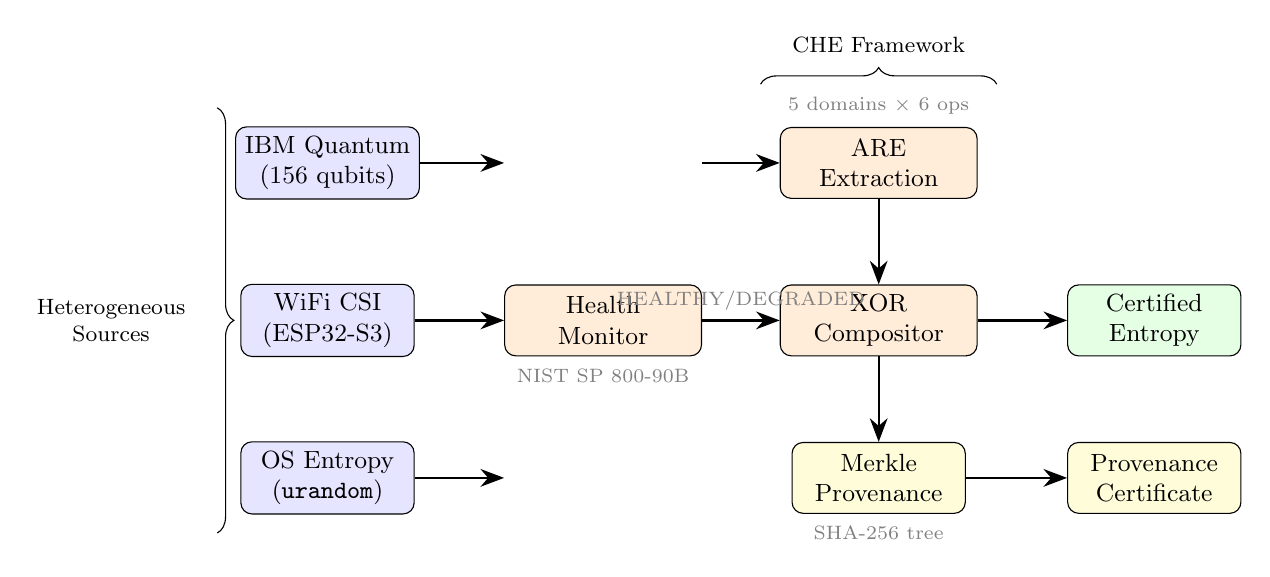
\begin{tikzpicture}[
  source/.style={draw, rounded corners, fill=blue!10, minimum width=2.2cm, minimum height=0.9cm, align=center, font=\small},
  process/.style={draw, rounded corners, fill=orange!15, minimum width=2.5cm, minimum height=0.9cm, align=center, font=\small},
  output/.style={draw, rounded corners, fill=green!10, minimum width=2.2cm, minimum height=0.9cm, align=center, font=\small},
  cert/.style={draw, rounded corners, fill=yellow!15, minimum width=2.2cm, minimum height=0.9cm, align=center, font=\small},
  arr/.style={-{Stealth[length=3mm]}, thick},
  label/.style={font=\scriptsize, text=gray},
]

% Entropy Sources (left column)
\node[source] (quantum) at (0, 2) {IBM Quantum\\(156 qubits)};
\node[source] (csi)     at (0, 0) {WiFi CSI\\(ESP32-S3)};
\node[source] (os)      at (0,-2) {OS Entropy\\(\texttt{urandom})};

% Health monitoring
\node[process] (health) at (3.5, 0) {Health\\Monitor};

% ARE Extraction
\node[process] (are) at (7, 2) {ARE\\Extraction};

% XOR Compositor
\node[process] (xor) at (7, 0) {XOR\\Compositor};

% Provenance
\node[cert] (merkle) at (7, -2) {Merkle\\Provenance};

% Output
\node[output] (output) at (10.5, 0) {Certified\\Entropy};

% Certificate
\node[cert] (certificate) at (10.5, -2) {Provenance\\Certificate};

% Arrows: sources -> health
\draw[arr] (quantum.east) -- (health.west |- quantum.east);
\draw[arr] (csi.east) -- (health.west);
\draw[arr] (os.east) -- (health.west |- os.east);

% Arrows: health -> compositor
\draw[arr] (health.east) -- node[above, label] {HEALTHY/DEGRADED} (xor.west);
\draw[arr] (health.east |- quantum.east) -- (are.west);

% Arrows: ARE -> compositor
\draw[arr] (are.south) -- (xor.north);

% Arrows: compositor -> output
\draw[arr] (xor.east) -- (output.west);

% Arrows: compositor -> merkle
\draw[arr] (xor.south) -- (merkle.north);

% Arrows: merkle -> certificate
\draw[arr] (merkle.east) -- (certificate.west);

% Brace for sources
\draw[decorate, decoration={brace, amplitude=6pt, mirror}] (-1.4, -2.7) -- (-1.4, 2.7) node[midway, left=8pt, align=center, font=\footnotesize] {Heterogeneous\\Sources};

% Brace for CHE framework
\draw[decorate, decoration={brace, amplitude=6pt}] (5.5, 3) -- (8.5, 3) node[midway, above=8pt, align=center, font=\footnotesize] {CHE Framework};

% Labels
\node[label, below=1pt] at (health.south) {NIST SP 800-90B};
\node[label, above=1pt] at (are.north) {5 domains $\times$ 6 ops};
\node[label, below=1pt] at (merkle.south) {SHA-256 tree};

\end{tikzpicture}
\end{document}
